%%%%%%%%%%%%%%%%%%%%%%%%%%%%%%%%%%%%%%%%%%%%%%%%%%%%%%%%%%%%%%%%%%%%%%%%
% Plantilla TFG/TFM
% Escuela Politécnica Superior de la Universidad de Alicante
% Realizado por: Jose Manuel Requena Plens
% Contacto: info@jmrplens.com / Telegram:@jmrplens
%%%%%%%%%%%%%%%%%%%%%%%%%%%%%%%%%%%%%%%%%%%%%%%%%%%%%%%%%%%%%%%%%%%%%%%%

\chapter{Estudio viabilidad}
\label{estudioviabilidad}
En este punto del proyecto se va a presentar una planificación temporal del proyecto, la planificación de los recursos y requisitos, además de una planificación de riesgos.
\subsection{Planificación temporal}
Para llegar a buen puerto en un proyecto es necesario intentar una buena estimación, que sabiendo que no es tarea fácil y difícil de cumplir, teniendo fechas de entrega continua al cliente podemos establecer prioridades y tomar decisiones estructurales en función de las necesidades temporales y de entrega. Como puede ser, por ejemplo, la entrada de nuevos requisitos que hacen retroceder otras funcionalidades en prioridad o que, incluso, las hacen quedar fuera del backlog; o que por problemas técnicos o por dificultad de implementación una tarea se retrase tanto que arrastre otras relacionadas.
\vspace{1em}
\par Cada hito realizado se asemeja bastante a las fases de la ingeniería de software y, a grandes rasgos, son los siguientes:
\begin{itemize}
    \item Hito 0 - Análisis:
    En este primer hito se realiza la primera ronda de contacto con los temas relacionados del proyecto. En este proyecto han sido el estudio de la disponibilidad web low-cost y acercarnos al banco de alimentos a ver en vivo el trabajo y necesidades de los voluntarios.
    \item Hito 1 - Especificación:
    En este hito se realizan los estudios y la documentación tanto del estado del arte como de las herramientas a utilizar. Además, se especifican los requisitos, los riesgos y se documentan los casos de uso y los diagramas.
    \item Hito 2 - Fase de desarrollo:
    Éste es el hito más largo y complicado, consiste en realizar el desarrollo del la apliacción backend, diseño e implementación de bases de datos y desarrollo del frontend.
    \item Hito 3 - Fase de pruebas:
    Último hito, en este se realizan pruebas de integración y satisfaccción además de revisar y finalizar la memoria.
\end{itemize}
\vspace{1em}
\par En este proyecto la planificación temporal empezó una vez llegados al hito 2, se ha usado la funcionalidad de Canvan, Issues y Milestone que proporciona Github en su plataforma.
\begin{figure}[h]
\centering
\begin{tabular}{ccc}
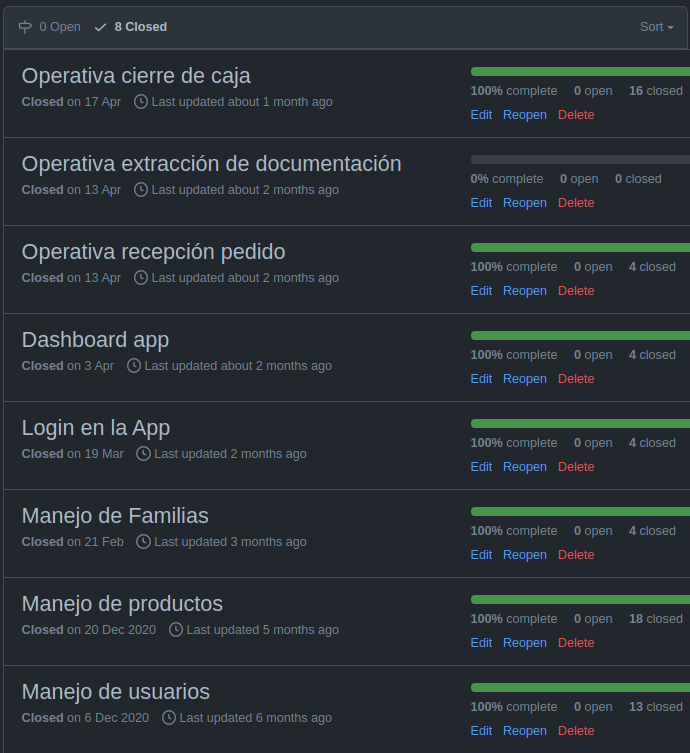
\includegraphics[scale=0.62]{archivos/github_milestones.png}
\end{tabular}
\caption{Milestones cerradas en Github}
\label{fig:github_milestones}
\end{figure}
\clearpage
\subsection{Gestión de riesgos}